\documentclass[ignorenonframetext,notheorems,aspectratio=1610]{beamer}
\usetheme[compress]{Madrid}
\usecolortheme{iwr}
\usepackage{../mathsim}
\mathtoolsset{showonlyrefs}

\externaldocument{main}

\makeatletter
\def\BT@with[#1]#2(#3){\begin{block}{#3 \capitalizewords{#2} (#1)}}
\def\BT@without#1(#2){\begin{block}{#2 \capitalizewords{#1}}}
\def\endblocktheorem{\end{block}}
\makeatother
\def\mylabel#1{}
\let\label\mylabel
%\renewcommand{\label}[1]{}

\begin{document}
\frame{\tableofcontents}
\section{Examples for mixed problems}
\frame {\input {blocks/Notation-vector-diff-operators.tex}}
\frame {\input {blocks/Definition-strain-tensor.tex}}
\frame {\input {blocks/Definition-hooke.tex}}
\frame {\input {blocks/Definition-weak-lame-navier.tex}}
\frame {\input {blocks/Problem-frobenius.tex}}
\frame {\input {blocks/Assumption-korn-inequality.tex}}
\frame {\input {blocks/Lemma-korn.tex}}
\frame {\input {blocks/Problem-elasticity-standard.tex}}

\begin{frame}
  \frametitle{Example: hanging sheet}
  \centering
  \begin{tabular}{ccc}
    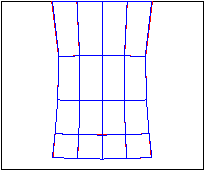
\includegraphics[width=.25\textwidth]{./graph/elasticity/stalactite-0}
    &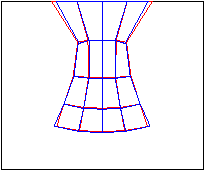
\includegraphics[width=.25\textwidth]{./graph/elasticity/stalactite-1}
    &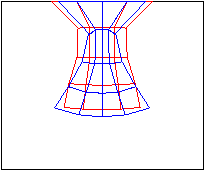
\includegraphics[width=.25\textwidth]{./graph/elasticity/stalactite-2}
    \\
    $\lambda = 1$&$\lambda = 10$&$\lambda = 100$
    \\\\
    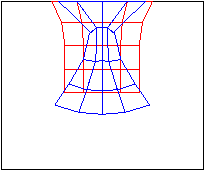
\includegraphics[width=.25\textwidth]{./graph/elasticity/stalactite-3}
    &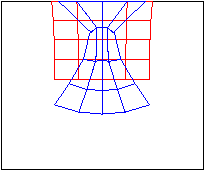
\includegraphics[width=.25\textwidth]{./graph/elasticity/stalactite-4}
    &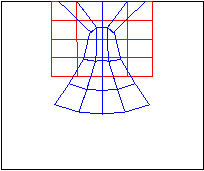
\includegraphics[width=.25\textwidth]{./graph/elasticity/stalactite-5}
    \\
    $\lambda = 1000$&$\lambda = 10000$&$\lambda = 100000$
  \end{tabular}
\end{frame}
\frame {\input {blocks/Definition-displacement-pressure.tex}}
\frame {\input {blocks/Definition-lame-navier-strong.tex}}
\frame {\input {blocks/Definition-saddle-point-operators.tex}}
\frame {\input {blocks/Definition-saddle-point-abstract.tex}}
\frame {\input {blocks/Notation-saddle-point-form.tex}}
\frame {\input {blocks/Definition-schur-complement.tex}}
\frame {\input {blocks/Lemma-schur-complement1.tex}}
\frame {\input {blocks/Lemma-schur-definiteness.tex}}
\frame {\input {blocks/Definition-stokes-eq1.tex}}
\frame {\input {blocks/Definition-solenoidal.tex}}
\frame {\input {blocks/Lemma-stokes-equivalence.tex}}
\frame {\input {blocks/Definition-stokes-eq2.tex}}
\frame {\input {blocks/Definition-stokes-boundary2.tex}}
\frame {\input {blocks/Lemma-divergence-compatibility.tex}}

\frame {\input {blocks/Theorem-la-invertible.tex}}
\frame {\input {blocks/Definition-infsup1.tex}}
\frame {\input {blocks/Lemma-infsup2.tex}}
\frame {\input {blocks/Theorem-infsup-well-posedness.tex}}
\end{document}
